This section is new in this report. Before comparing forecasters, it asks which properties of the RTT carry over from the 6\,s input window to the 3\,s forecast horizon. The answer explains the results of the following sections: why the RMSE hardly moves, why calibrated intervals improve so much, and why the gain differs between links. The statistics use the measured pings of the training sessions, with each session centered on its own mean so that differences between sessions do not appear as memory. Confidence intervals come from a bootstrap over sessions (script \texttt{fr\_volatility.py}).

\begin{figure}[H]
  \centering
  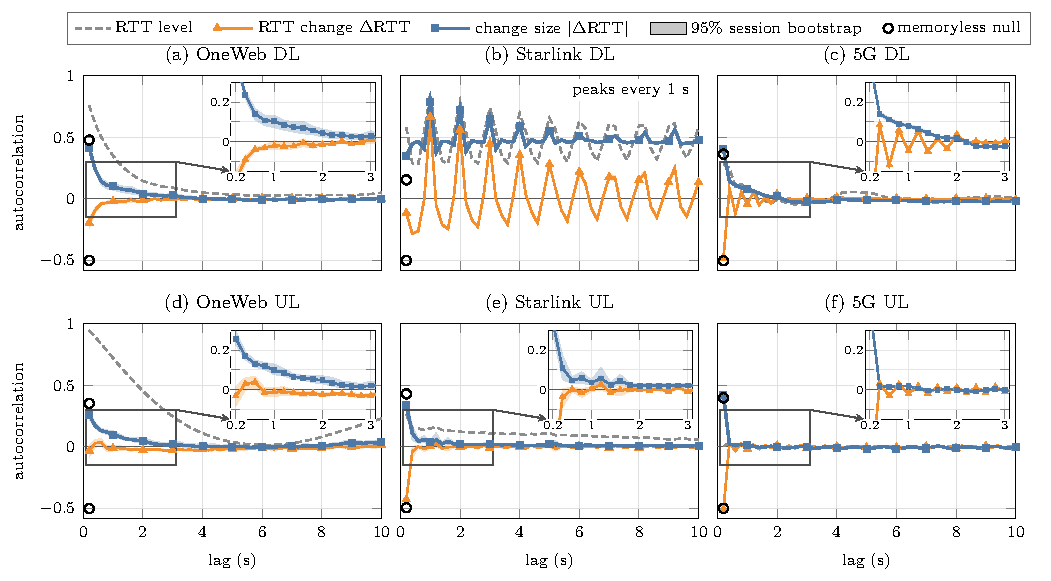
\includegraphics[width=\linewidth]{figs_pdf/fr_volatility.pdf}
  \caption{Autocorrelation of the RTT level, of its 200\,ms change $\Delta$RTT, and of the size of the change $|\Delta\mathrm{RTT}|$ in the training sessions (shaded: 95\% session-bootstrap interval). Circles: value of a memoryless series at 0.2\,s. A curve that starts on its circle has no memory at the first lag. Insets: lags of 0.2 to 3\,s. Starlink DL peaks every second because of a load-driven sawtooth.}
  \label{fig:vol}
\end{figure}

\paragraph{The next change is hard to predict, the level reverts.} Fig.~\ref{fig:vol} shows the autocorrelation of the RTT level, of its change between consecutive rows, and of the size of the change. At the first lag the change of a memoryless series has an autocorrelation of $-0.5$ (circles), because two consecutive changes share one sample. From 0.4\,s to 10\,s the autocorrelation of $\Delta$RTT stays within $\pm$\VolDmaxAbs{} on five links: past changes say almost nothing about the next change. The direction of the next change is still partly predictable, because the RTT returns toward its recent level. Expecting a return to the mean of the 6\,s input gets the sign of the 1\,s change right in \VolSignRevLo\% to \VolSignRevHi\% of the test windows (balanced accuracy, 50\% for a constant guess), and the learned forecasters reach \VolSignNNLo\% to \VolSignNNHi\%. Point forecasts thus beat persistence mainly by not repeating the last, noisy ping. Their MAE is \PersRatioLo{} to \PersRatioHi{} times lower than that of persistence, but none of them gets much closer to the actual next value than the others, which is why the RMSE hardly separates them.

\paragraph{The spread depends on the link state.} The size of the change has a short memory: its autocorrelation at 1\,s is \VolAbsdLo{} to \VolAbsdHi{} on OneWeb and 5G DL, and on the five links without a sawtooth it stays positive for 1.4 to 5.8\,s. Inside one session this memory is too weak to forecast the next seconds. On OneWeb and 5G, the standard deviation (SD) of the 6\,s input does not predict the error of a 1\,s forecast within a session (rank correlation \VolWithinLo{} to \VolWithinHi), but it does between sessions (\VolBetweenLo{} to \VolBetweenHi). Each session runs in a noise regime set by its load and radio conditions, and a few seconds of input reveal that regime. Starlink DL is different. Under the saturating downlink test its RTT climbs from about 35\,ms to about 200\,ms in steps of about 50\,ms and drops back once per second, which produces the peaks in Fig.~\ref{fig:vol}(b). The RTT autocorrelation at 1\,s is \VolSLDLlevel{} and exceeds \VolSLDLlevelMin{} in every one of the \VolSLDLnSess{} training sessions. The sawtooth switches on and off within a session (Fig.~\ref{fig:trace1min}), and the volatility of the last 6\,s predicts that of the next 3\,s (within-session rank correlation \VolSLDLrv). We attribute the sawtooth to queue build-up and drain under the saturating load, since the uplink test does not show it.

\paragraph{Errors are skewed upward.} The RTT moves up further than it moves down. Queues and retransmissions add delay, while nothing removes delay below the propagation floor. For the 1\,s forecasts of the previous model, the 97.5\% quantile of the error on the calibration sessions is \SkewQUL{} times the size of the 2.5\% quantile on 5G UL and \SkewOWDL{} times on OneWeb DL.

\paragraph{Consequence for uncertainty.} An interval of constant width around a point forecast, which is how the previous report attached uncertainty to its forecasts, ignores both properties. Calibrated to cover 95\% of all windows, it covers \CovConstCalmLo{} to \CovConstCalmHi{} of the calmest tenth of windows and \CovConstVolLo{} to \CovConstVolHi{} of the most volatile tenth. The calm windows are covered more often on every link. On Starlink DL the interval is \WidConstSLDL\,ms wide at 1\,s ahead in every window, while a quiet window rarely moves by more than a few milliseconds. The interval score is minimized by the conditional quantiles of the target~\cite{gneiting2007strictly}, so a forecaster should learn the spread and its skew from the input. Because the regime differs between sessions, its intervals must be calibrated on sessions it has not seen. Fig.~\ref{fig:trace1min} shows the result on one minute of a Starlink DL test session.

\begin{figure}[H]
  \centering
  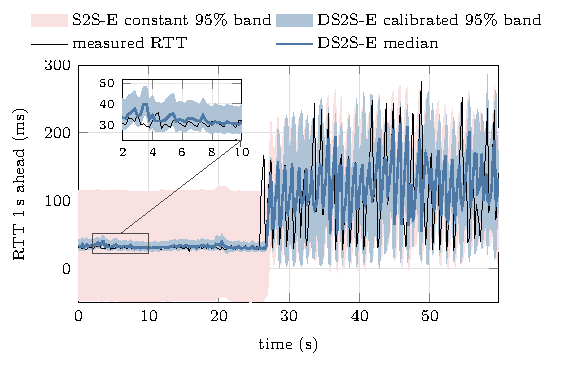
\includegraphics{figs_pdf/fr_trace.pdf}
  \caption{One minute of a Starlink DL test session, forecast 1\,s ahead. The previous model (S2S-E) has a constant 95\% interval of \TraceWidS\,ms. The calibrated interval of the final model (DS2S-E) is \TraceWidDCalm\,ms wide (median) while the link is quiet and \TraceWidDLoad\,ms once it swings. Inset: the quiet part.}
  \label{fig:trace1min}
\end{figure}
